\subsection{Sample scatter touched against commit - Repository: 21} 
\begin{figure}[!htbp]
  \centering 
  \hfill 
  \begin{subfigure}[b]{0.48\textwidth}
    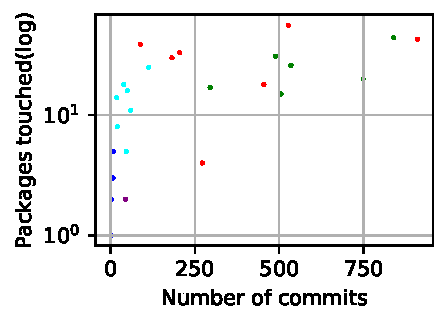
\includegraphics[width=\textwidth]{sections/results/21/packages/sample_scatter_touched_against_commit.packages.sample.first.pdf}
    \caption{packages}
    \label{figure.24.00000000000003}
  \end{subfigure}
  \vspace{0.5cm}
  \hfill 
  \begin{subfigure}[b]{0.48\textwidth}
    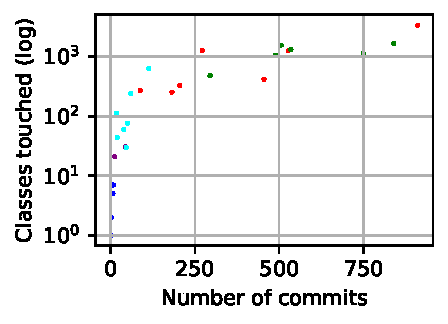
\includegraphics[width=\textwidth]{sections/results/21/classes/sample_scatter_touched_against_commit.classes.sample.first.pdf}
    \caption{classes}
    \label{figure.30.10000000000006}
  \end{subfigure}
  \hfill 
  \begin{subfigure}[b]{0.48\textwidth}
    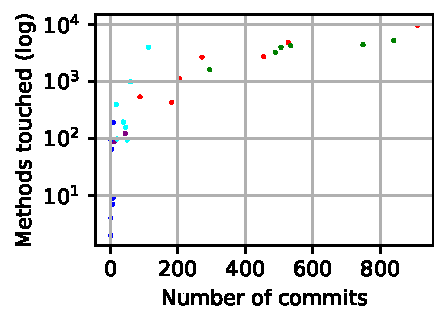
\includegraphics[width=\textwidth]{sections/results/21/methods/sample_scatter_touched_against_commit.methods.sample.first.pdf}
    \caption{methods}
    \label{figure.34.20000000000009}
  \end{subfigure}
\caption[Short]{\begin{minipage}[t]{\linewidth}Scatter plots of the log total number of components touched (y-axis) against the number of commits (x-axis) made by samples of developers capped at 84 sustained later joiners from six (6) categories: \color{Blue}Transient Founder (Blue, NUM1), \color{Purple}Moderate Founder (Purple, 3), \color{Green} Sustained Founder (Green, 7), \color{Orange} Transient Later Joiner (Orange, 84), \color{Cyan}Moderate Later Joiner (Cyan, 84), \color{Red} Sustained Later Joiner (Red, 84). \color{Black}\end{minipage}} 
  \hfill 
\end{figure}
\newpage 
\subsection{Sample scatter touched against commit - Repository: 21} 
\begin{figure}[!htbp]
  \centering 
  \begin{subfigure}[b]{0.48\textwidth}
    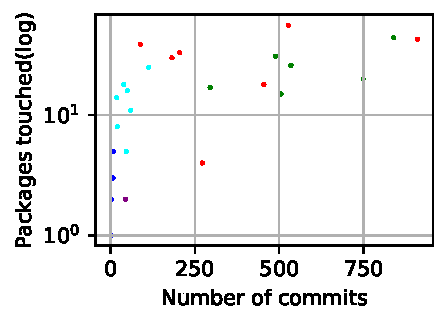
\includegraphics[width=\textwidth]{sections/results/21/packages/sample_scatter_touched_against_commit.packages.sample.first.pdf}
    \caption{packages}
    \label{figure.24.00000000000003}
  \end{subfigure}
  \vspace{0.5cm}
  \begin{subfigure}[b]{0.48\textwidth}
    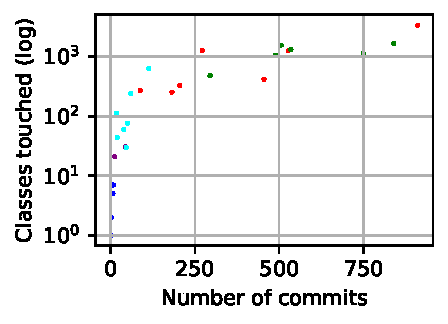
\includegraphics[width=\textwidth]{sections/results/21/classes/sample_scatter_touched_against_commit.classes.sample.first.pdf}
    \caption{classes}
    \label{figure.30.10000000000006}
  \end{subfigure}
  \begin{subfigure}[b]{0.48\textwidth}
    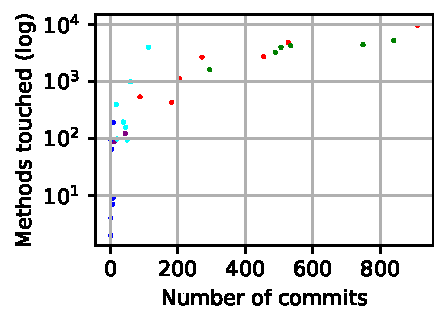
\includegraphics[width=\textwidth]{sections/results/21/methods/sample_scatter_touched_against_commit.methods.sample.first.pdf}
    \caption{methods}
    \label{figure.34.20000000000009}
  \end{subfigure}
\caption[Short]{\begin{minipage}[t]{\linewidth}Scatter plots of the log total number of components touched (y-axis) against the number of commits (x-axis) made by samples of developers capped at 84 sustained later joiners from six (6) categories: \color{Blue}Transient Founder (Blue, NUM1), \color{Purple}Moderate Founder (Purple, 3), \color{Green} Sustained Founder (Green, 7), \color{Orange} Transient Later Joiner (Orange, 84), \color{Cyan}Moderate Later Joiner (Cyan, 84), \color{Red} Sustained Later Joiner (Red, 84). \color{Black}\end{minipage}} 
  \hfill 
\end{figure}
\newpage 
\subsection{Sample scatter touched against commit - Repository: 21} 
\begin{figure}[!htbp]
  \centering 
  \begin{subfigure}[b]{0.48\textwidth}
    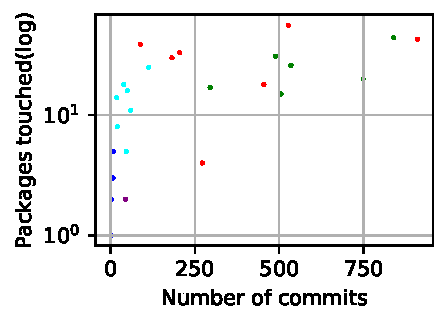
\includegraphics[width=\textwidth]{sections/results/21/packages/sample_scatter_touched_against_commit.packages.sample.first.pdf}
    \caption{packages}
    \label{figure.24.00000000000003
}
  \end{subfigure}%
  \vspace{0.5cm}
  \begin{subfigure}[b]{0.48\textwidth}
    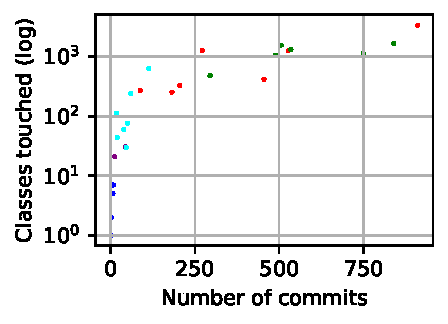
\includegraphics[width=\textwidth]{sections/results/21/classes/sample_scatter_touched_against_commit.classes.sample.first.pdf}
    \caption{classes}
    \label{figure.30.10000000000006
}
  \end{subfigure}%
  \begin{subfigure}[b]{0.48\textwidth}
    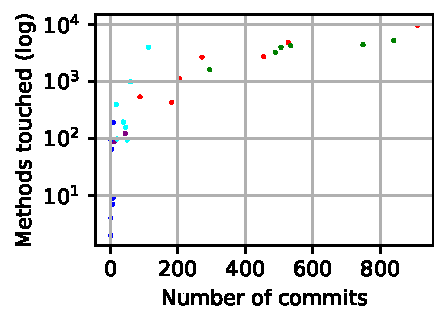
\includegraphics[width=\textwidth]{sections/results/21/methods/sample_scatter_touched_against_commit.methods.sample.first.pdf}
    \caption{methods}
    \label{figure.34.20000000000009
}
  \end{subfigure}%
\caption[Short]{\begin{minipage}[t]{\linewidth}Scatter plots of the log total number of components touched (y-axis) against the number of commits (x-axis) made by samples of developers capped at 84 sustained later joiners from six (6) categories: \color{Blue}Transient Founder (Blue, NUM1), \color{Purple}Moderate Founder (Purple, 3), \color{Green} Sustained Founder (Green, 7), \color{Orange} Transient Later Joiner (Orange, 84), \color{Cyan}Moderate Later Joiner (Cyan, 84), \color{Red} Sustained Later Joiner (Red, 84). \color{Black}\end{minipage}} 
  \hfill 
\end{figure}
\newpage 
\subsection{Sample scatter touched against commit - Repository: 21} 
\begin{figure}[!htbp]
  \centering 
  \begin{subfigure}[b]{0.48\textwidth}
    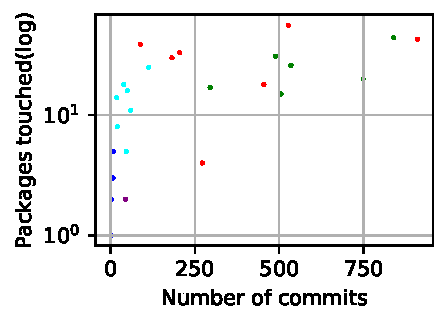
\includegraphics[width=\textwidth]{sections/results/21/packages/sample_scatter_touched_against_commit.packages.sample.first.pdf}
    \caption{packages}
    \label{figure.24.00000000000003}
  \end{subfigure}%
  \vspace{0.5cm}
  \begin{subfigure}[b]{0.48\textwidth}
    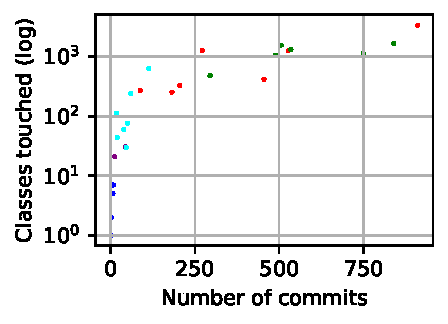
\includegraphics[width=\textwidth]{sections/results/21/classes/sample_scatter_touched_against_commit.classes.sample.first.pdf}
    \caption{classes}
    \label{figure.30.10000000000006}
  \end{subfigure}%
  \begin{subfigure}[b]{0.48\textwidth}
    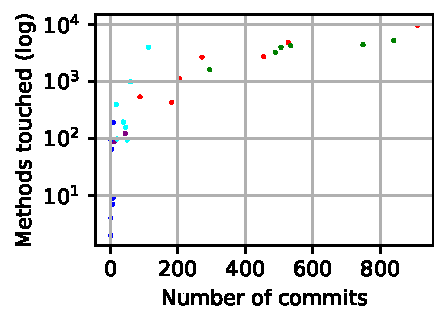
\includegraphics[width=\textwidth]{sections/results/21/methods/sample_scatter_touched_against_commit.methods.sample.first.pdf}
    \caption{methods}
    \label{figure.34.20000000000009}
  \end{subfigure}%
\caption[Short]{\begin{minipage}[t]{\linewidth}Scatter plots of the log total number of components touched (y-axis) against the number of commits (x-axis) made by samples of developers capped at 84 sustained later joiners from six (6) categories: \color{Blue}Transient Founder (Blue, NUM1), \color{Purple}Moderate Founder (Purple, 3), \color{Green} Sustained Founder (Green, 7), \color{Orange} Transient Later Joiner (Orange, 84), \color{Cyan}Moderate Later Joiner (Cyan, 84), \color{Red} Sustained Later Joiner (Red, 84). \color{Black}\end{minipage}} 
  \hfill 
\end{figure}
\newpage 
\subsection{Sample scatter touched against commit - Repository: 21} 
\begin{figure}[!htbp]
  \centering 
  \begin{subfigure}[b]{0.48\textwidth}
    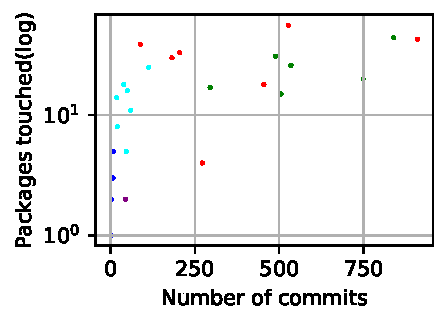
\includegraphics[width=\textwidth]{sections/results/21/packages/sample_scatter_touched_against_commit.packages.sample.first.pdf}
    \caption{packages}
    \label{figure.24.00000000000003}
  \end{subfigure}%
  \vspace{0.5cm}
  \begin{subfigure}[b]{0.48\textwidth}
    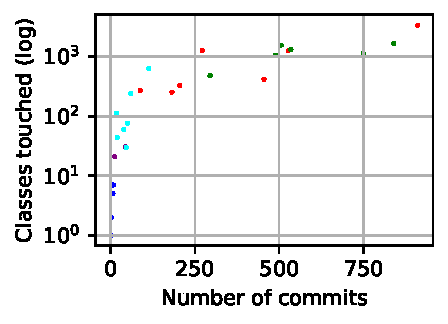
\includegraphics[width=\textwidth]{sections/results/21/classes/sample_scatter_touched_against_commit.classes.sample.first.pdf}
    \caption{classes}
    \label{figure.30.10000000000006}
  \end{subfigure}%
  \begin{subfigure}[b]{0.48\textwidth}
    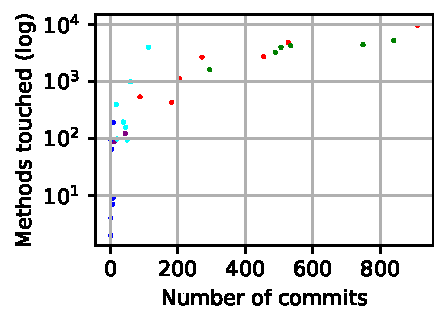
\includegraphics[width=\textwidth]{sections/results/21/methods/sample_scatter_touched_against_commit.methods.sample.first.pdf}
    \caption{methods}
    \label{figure.34.20000000000009}
  \end{subfigure}%
\caption[Short]{\begin{minipage}[t]{\linewidth}Scatter plots of the log total number of components touched (y-axis) against the number of commits (x-axis) made by samples of developers capped at 84 sustained later joiners from six (6) categories: \color{Blue}Transient Founder (Blue, NUM1), \color{Purple}Moderate Founder (Purple, 3), \color{Green} Sustained Founder (Green, 7), \color{Orange} Transient Later Joiner (Orange, 84), \color{Cyan}Moderate Later Joiner (Cyan, 84), \color{Red} Sustained Later Joiner (Red, 84). \color{Black}\end{minipage}} 
\end{figure}
\newpage 
\subsection{Sample scatter touched against commit - Repository: 21} 
\begin{figure}[!htbp]
  \centering 
  \begin{subfigure}[b]    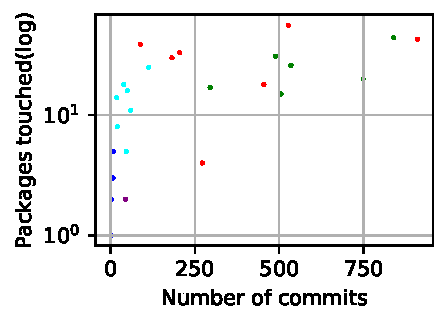
\includegraphics[width=0.45\linewidth]{sections/results/21/packages/sample_scatter_touched_against_commit.packages.sample.first.pdf}
    \caption{packages}
    \label{figure.24.00000000000003}
  \end{subfigure}%
  \vspace{0.5cm}
  \begin{subfigure}[b]    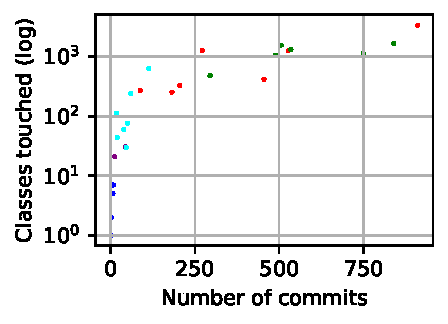
\includegraphics[width=0.45\linewidth]{sections/results/21/classes/sample_scatter_touched_against_commit.classes.sample.first.pdf}
    \caption{classes}
    \label{figure.30.10000000000006}
  \end{subfigure}%
  \begin{subfigure}[b]    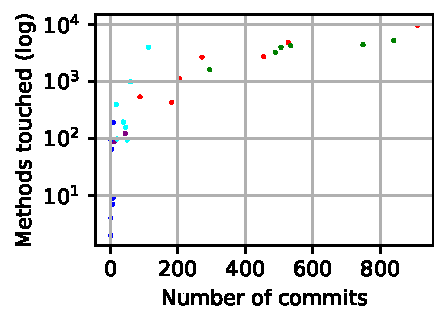
\includegraphics[width=0.45\linewidth]{sections/results/21/methods/sample_scatter_touched_against_commit.methods.sample.first.pdf}
    \caption{methods}
    \label{figure.34.20000000000009}
  \end{subfigure}%
\caption[Short]{\begin{minipage}[t]{\linewidth}Scatter plots of the log total number of components touched (y-axis) against the number of commits (x-axis) made by samples of developers capped at 84 sustained later joiners from six (6) categories: \color{Blue}Transient Founder (Blue, NUM1), \color{Purple}Moderate Founder (Purple, 3), \color{Green} Sustained Founder (Green, 7), \color{Orange} Transient Later Joiner (Orange, 84), \color{Cyan}Moderate Later Joiner (Cyan, 84), \color{Red} Sustained Later Joiner (Red, 84). \color{Black}\end{minipage}} 
\end{figure}
\newpage 
\subsection{Sample scatter touched against commit - Repository: 21} 
\begin{figure}[!htbp]
  \centering 
  \begin{subfigure}[b]
    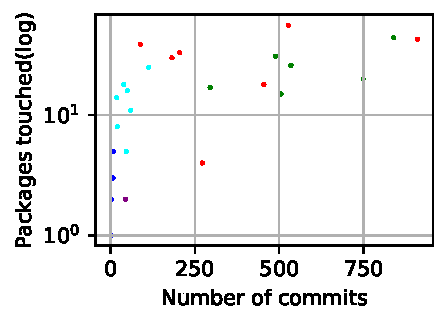
\includegraphics[width=0.45\linewidth]{sections/results/21/packages/sample_scatter_touched_against_commit.packages.sample.first.pdf}
    \caption{packages}
    \label{figure.24.00000000000003}
  \end{subfigure}%
  \vspace{0.5cm}
  \begin{subfigure}[b]
    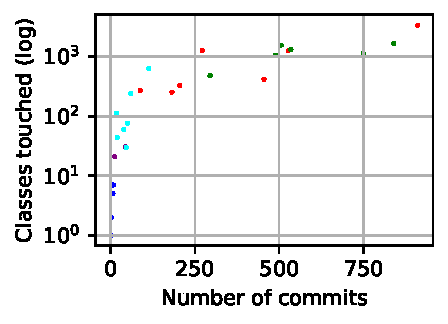
\includegraphics[width=0.45\linewidth]{sections/results/21/classes/sample_scatter_touched_against_commit.classes.sample.first.pdf}
    \caption{classes}
    \label{figure.30.10000000000006}
  \end{subfigure}%
  \begin{subfigure}[b]
    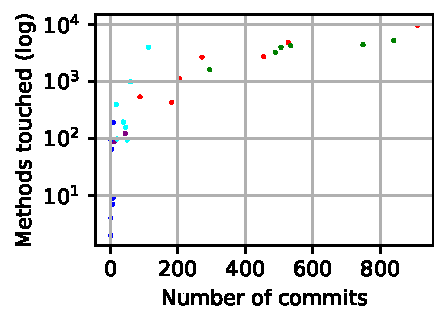
\includegraphics[width=0.45\linewidth]{sections/results/21/methods/sample_scatter_touched_against_commit.methods.sample.first.pdf}
    \caption{methods}
    \label{figure.34.20000000000009}
  \end{subfigure}%
\caption[Short]{\begin{minipage}[t]{\linewidth}Scatter plots of the log total number of components touched (y-axis) against the number of commits (x-axis) made by samples of developers capped at 84 sustained later joiners from six (6) categories: \color{Blue}Transient Founder (Blue, NUM1), \color{Purple}Moderate Founder (Purple, 3), \color{Green} Sustained Founder (Green, 7), \color{Orange} Transient Later Joiner (Orange, 84), \color{Cyan}Moderate Later Joiner (Cyan, 84), \color{Red} Sustained Later Joiner (Red, 84). \color{Black}\end{minipage}} 
\end{figure}
\newpage 
\subsection{Sample scatter touched against commit - Repository: 21} 
\begin{figure}[!htbp]
  \centering 
  \begin{subfigure}[b]{0.45\linewidth}
    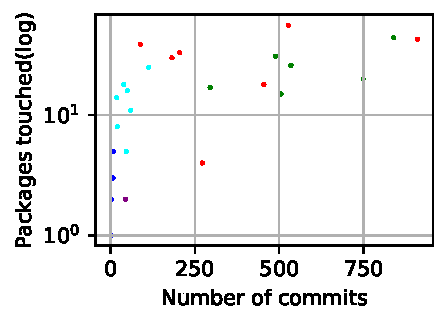
\includegraphics[width=0.45\linewidth]{sections/results/21/packages/sample_scatter_touched_against_commit.packages.sample.first.pdf}
    \caption{packages}
    \label{figure.24.00000000000003}
  \end{subfigure}%
  \vspace{0.5cm}
  \begin{subfigure}[b]{0.45\linewidth}
    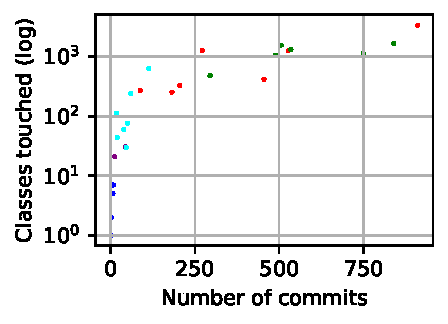
\includegraphics[width=0.45\linewidth]{sections/results/21/classes/sample_scatter_touched_against_commit.classes.sample.first.pdf}
    \caption{classes}
    \label{figure.30.10000000000006}
  \end{subfigure}%
  \begin{subfigure}[b]{0.45\linewidth}
    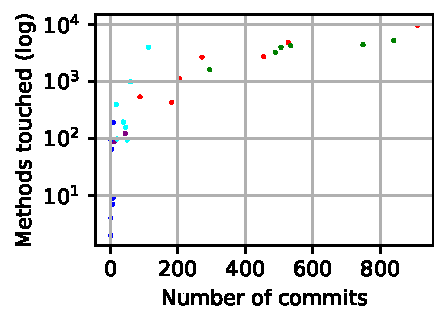
\includegraphics[width=0.45\linewidth]{sections/results/21/methods/sample_scatter_touched_against_commit.methods.sample.first.pdf}
    \caption{methods}
    \label{figure.34.20000000000009}
  \end{subfigure}%
\caption[Short]{\begin{minipage}[t]{\linewidth}Scatter plots of the log total number of components touched (y-axis) against the number of commits (x-axis) made by samples of developers capped at 84 sustained later joiners from six (6) categories: \color{Blue}Transient Founder (Blue, NUM1), \color{Purple}Moderate Founder (Purple, 3), \color{Green} Sustained Founder (Green, 7), \color{Orange} Transient Later Joiner (Orange, 84), \color{Cyan}Moderate Later Joiner (Cyan, 84), \color{Red} Sustained Later Joiner (Red, 84). \color{Black}\end{minipage}} 
\end{figure}
\newpage 
\subsection{Sample scatter touched against commit - Repository: 21} 
\begin{figure}[!htbp]
  \centering 
  \subfloat[packages\label{figure.24.00000000000003}]{%
    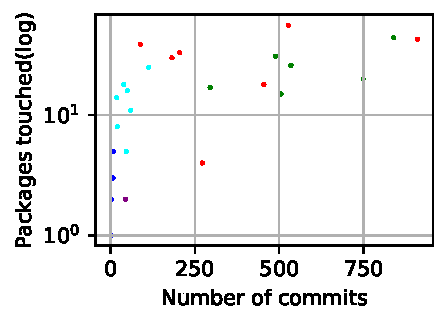
\includegraphics[width=0.45\linewidth]{sections/results/21/packages/sample_scatter_touched_against_commit.packages.sample.first.pdf}
}
  \vfill
  \subfloat[classes\label{figure.30.10000000000006}]{%
    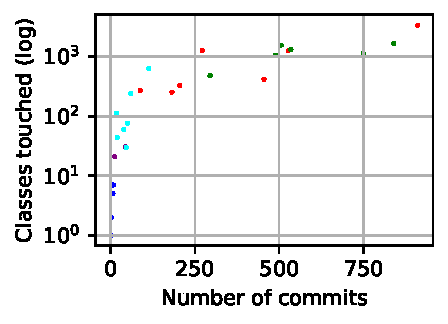
\includegraphics[width=0.45\linewidth]{sections/results/21/classes/sample_scatter_touched_against_commit.classes.sample.first.pdf}
}
  \subfloat[methods\label{figure.34.20000000000009}]{%
    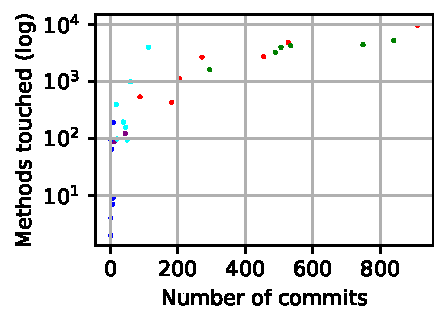
\includegraphics[width=0.45\linewidth]{sections/results/21/methods/sample_scatter_touched_against_commit.methods.sample.first.pdf}
}
\caption[Short]{\begin{minipage}[t]{\linewidth}Scatter plots of the log total number of components touched (y-axis) against the number of commits (x-axis) made by samples of developers capped at 84 sustained later joiners from six (6) categories: \color{Blue}Transient Founder (Blue, NUM1), \color{Purple}Moderate Founder (Purple, 3), \color{Green} Sustained Founder (Green, 7), \color{Orange} Transient Later Joiner (Orange, 84), \color{Cyan}Moderate Later Joiner (Cyan, 84), \color{Red} Sustained Later Joiner (Red, 84). \color{Black}\end{minipage}} 
\end{figure}
\newpage 
\subsection{Sample scatter touched against commit - Repository: 21} 
\begin{figure}[!htbp]
  \centering 
  \subfloat[packages\label{figure.24.00000000000003}]{%
    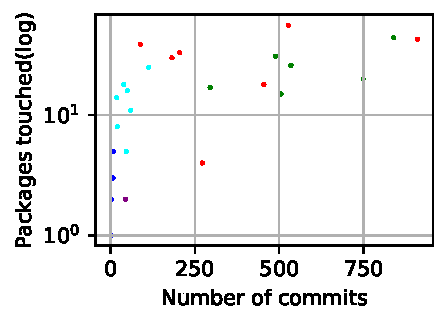
\includegraphics[width=0.45\linewidth]{sections/results/21/packages/sample_scatter_touched_against_commit.packages.sample.first.pdf}
    \caption{packages}
}
  \vfill
  \subfloat[classes\label{figure.30.10000000000006}]{%
    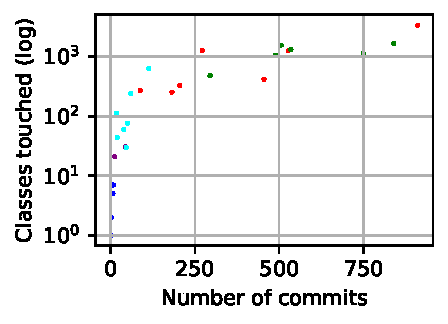
\includegraphics[width=0.45\linewidth]{sections/results/21/classes/sample_scatter_touched_against_commit.classes.sample.first.pdf}
    \caption{classes}
}
  \subfloat[methods\label{figure.34.20000000000009}]{%
    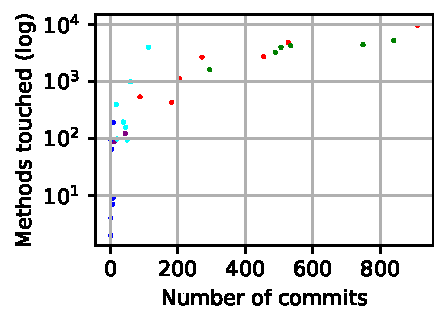
\includegraphics[width=0.45\linewidth]{sections/results/21/methods/sample_scatter_touched_against_commit.methods.sample.first.pdf}
    \caption{methods}
}
\caption[Short]{\begin{minipage}[t]{\linewidth}Scatter plots of the log total number of components touched (y-axis) against the number of commits (x-axis) made by samples of developers capped at 84 sustained later joiners from six (6) categories: \color{Blue}Transient Founder (Blue, NUM1), \color{Purple}Moderate Founder (Purple, 3), \color{Green} Sustained Founder (Green, 7), \color{Orange} Transient Later Joiner (Orange, 84), \color{Cyan}Moderate Later Joiner (Cyan, 84), \color{Red} Sustained Later Joiner (Red, 84). \color{Black}\end{minipage}} 
\end{figure}
\newpage 
\subsection{Sample scatter touched against commit - Repository: 21} 
\begin{figure}[!htbp]
  \centering 
  \subfloat[packages\label{figure.24.00000000000003}]{%
    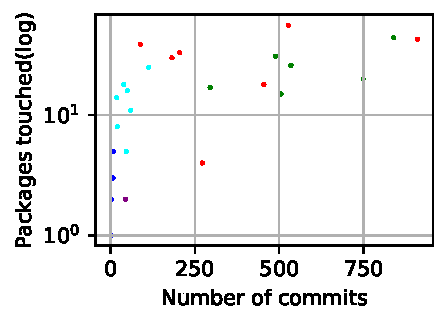
\includegraphics[width=0.45\linewidth]{sections/results/21/packages/sample_scatter_touched_against_commit.packages.sample.first.pdf}
}
  \vfill
  \subfloat[classes\label{figure.30.10000000000006}]{%
    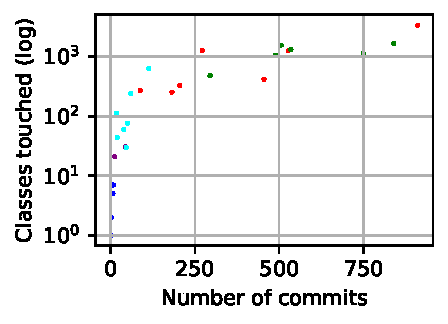
\includegraphics[width=0.45\linewidth]{sections/results/21/classes/sample_scatter_touched_against_commit.classes.sample.first.pdf}
}
  \subfloat[methods\label{figure.34.20000000000009}]{%
    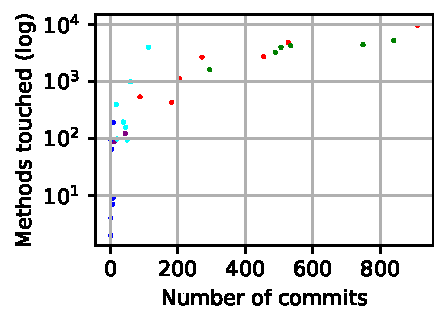
\includegraphics[width=0.45\linewidth]{sections/results/21/methods/sample_scatter_touched_against_commit.methods.sample.first.pdf}
}
\caption[Short]{\begin{minipage}[t]{\linewidth}Scatter plots of the log total number of components touched (y-axis) against the number of commits (x-axis) made by samples of developers capped at 84 sustained later joiners from six (6) categories: \color{Blue}Transient Founder (Blue, NUM1), \color{Purple}Moderate Founder (Purple, 3), \color{Green} Sustained Founder (Green, 7), \color{Orange} Transient Later Joiner (Orange, 84), \color{Cyan}Moderate Later Joiner (Cyan, 84), \color{Red} Sustained Later Joiner (Red, 84). \color{Black}\end{minipage}} 
\end{figure}
\newpage 
\subsection{Sample scatter touched against commit - Repository: 21} 
\begin{figure}[!htbp]
  \centering 
  \hfill 
  \\begin{minipage}[b] 
{0.45\textwidth}
    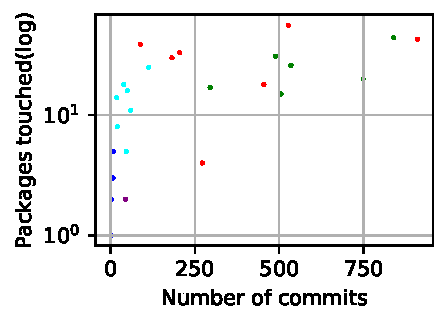
\includegraphics[width=	extwidth]{sections/results/21/packages/sample_scatter_touched_against_commit.packages.sample.first.pdf}
    \caption{packages}
    \label{figure.24.00000000000003}
  \\end{minipage}\n  \vfill
  \hfill 
  \\begin{minipage}[b] 
{0.45\textwidth}
    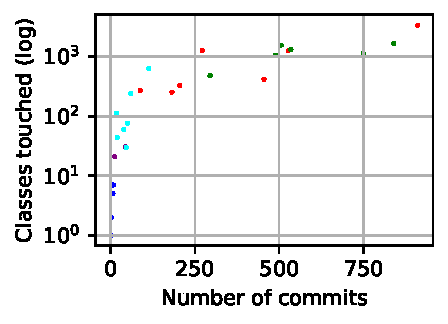
\includegraphics[width=	extwidth]{sections/results/21/classes/sample_scatter_touched_against_commit.classes.sample.first.pdf}
    \caption{classes}
    \label{figure.30.10000000000006}
  \\end{minipage}\n  \hfill 
  \\begin{minipage}[b] 
{0.45\textwidth}
    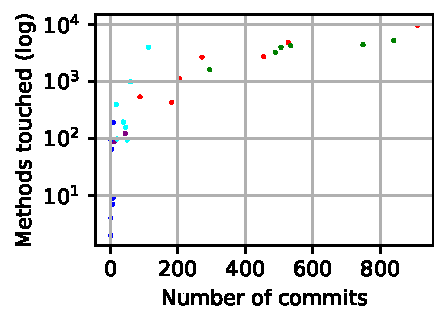
\includegraphics[width=	extwidth]{sections/results/21/methods/sample_scatter_touched_against_commit.methods.sample.first.pdf}
    \caption{methods}
    \label{figure.34.20000000000009}
  \\end{minipage}\n\caption[Short]{\begin{minipage}[t]{\linewidth}Scatter plots of the log total number of components touched (y-axis) against the number of commits (x-axis) made by samples of developers capped at 84 sustained later joiners from six (6) categories: \color{Blue}Transient Founder (Blue, NUM1), \color{Purple}Moderate Founder (Purple, 3), \color{Green} Sustained Founder (Green, 7), \color{Orange} Transient Later Joiner (Orange, 84), \color{Cyan}Moderate Later Joiner (Cyan, 84), \color{Red} Sustained Later Joiner (Red, 84). \color{Black}\end{minipage}} 
\end{figure}
\newpage 
\subsection{Sample scatter touched against commit - Repository: 21} 
\begin{figure}[!htbp]
  \centering 
  \hfill 
  \begin{minipage}[b]{0.45\textwidth}

    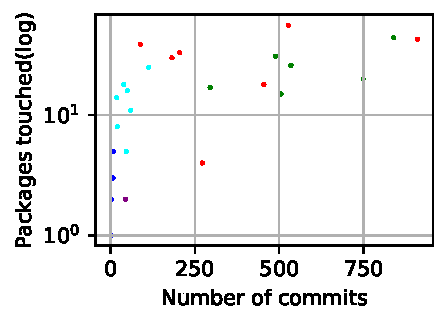
\includegraphics[width=	extwidth]{sections/results/21/packages/sample_scatter_touched_against_commit.packages.sample.first.pdf}
\vskip 5pt
    {packages}
    \label{figure.24.00000000000003}
  \end{minipage}%\n  \vfill
  \hfill 
  \begin{minipage}[b]{0.45\textwidth}

    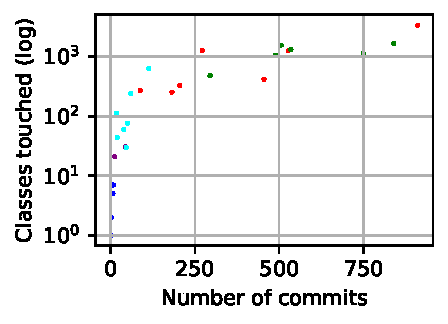
\includegraphics[width=	extwidth]{sections/results/21/classes/sample_scatter_touched_against_commit.classes.sample.first.pdf}
\vskip 5pt
    {classes}
    \label{figure.30.10000000000006}
  \end{minipage}%\n  \hfill 
  \begin{minipage}[b]{0.45\textwidth}

    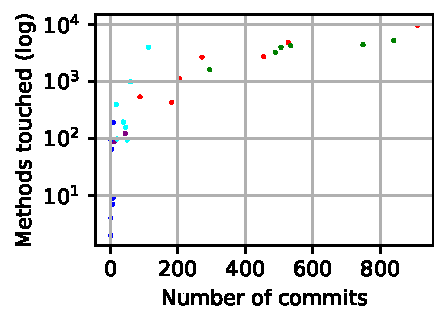
\includegraphics[width=	extwidth]{sections/results/21/methods/sample_scatter_touched_against_commit.methods.sample.first.pdf}
\vskip 5pt
    {methods}
    \label{figure.34.20000000000009}
  \end{minipage}%\n\caption[Short]{\begin{minipage}[t]{\linewidth}Scatter plots of the log total number of components touched (y-axis) against the number of commits (x-axis) made by samples of developers capped at 84 sustained later joiners from six (6) categories: \color{Blue}Transient Founder (Blue, NUM1), \color{Purple}Moderate Founder (Purple, 3), \color{Green} Sustained Founder (Green, 7), \color{Orange} Transient Later Joiner (Orange, 84), \color{Cyan}Moderate Later Joiner (Cyan, 84), \color{Red} Sustained Later Joiner (Red, 84). \color{Black}\end{minipage}} 
\end{figure}
\newpage 
\subsection{Sample scatter touched against commit - Repository: 21} 
\begin{figure}[!htbp]
  \centering 
  \hfill 
  \begin{minipage}[b]{0.45\textwidth}

    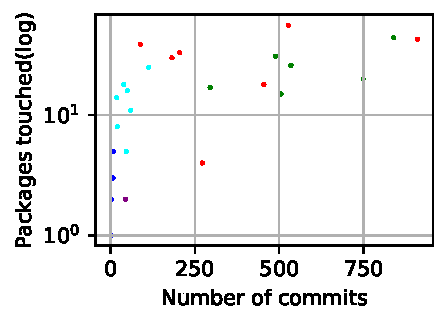
\includegraphics[width=\textwidth]{sections/results/21/packages/sample_scatter_touched_against_commit.packages.sample.first.pdf}
    \vskip 5pt
    {packages}
    \label{figure.24.00000000000003}
  \end{minipage}%\n  \vfill
  \hfill 
  \begin{minipage}[b]{0.45\textwidth}

    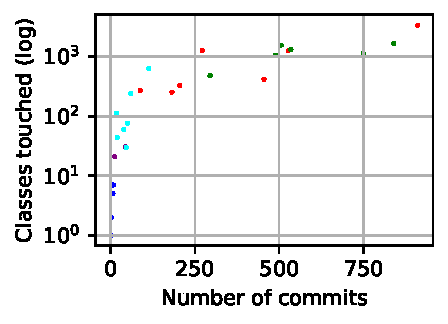
\includegraphics[width=\textwidth]{sections/results/21/classes/sample_scatter_touched_against_commit.classes.sample.first.pdf}
    \vskip 5pt
    {classes}
    \label{figure.30.10000000000006}
  \end{minipage}%\n  \hfill 
  \begin{minipage}[b]{0.45\textwidth}

    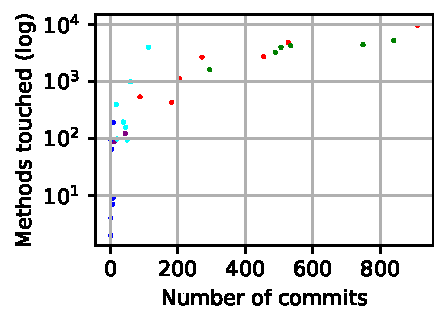
\includegraphics[width=\textwidth]{sections/results/21/methods/sample_scatter_touched_against_commit.methods.sample.first.pdf}
    \vskip 5pt
    {methods}
    \label{figure.34.20000000000009}
  \end{minipage}%\n\caption[Short]{\begin{minipage}[t]{\linewidth}Scatter plots of the log total number of components touched (y-axis) against the number of commits (x-axis) made by samples of developers capped at 84 sustained later joiners from six (6) categories: \color{Blue}Transient Founder (Blue, NUM1), \color{Purple}Moderate Founder (Purple, 3), \color{Green} Sustained Founder (Green, 7), \color{Orange} Transient Later Joiner (Orange, 84), \color{Cyan}Moderate Later Joiner (Cyan, 84), \color{Red} Sustained Later Joiner (Red, 84). \color{Black}\end{minipage}} 
\end{figure}
\newpage 
\subsection{Sample scatter touched against commit - Repository: 21} 
\begin{figure}[!htbp]
  \centering 
\begin{minipage}[b]({0.45\textwidth})
\centering
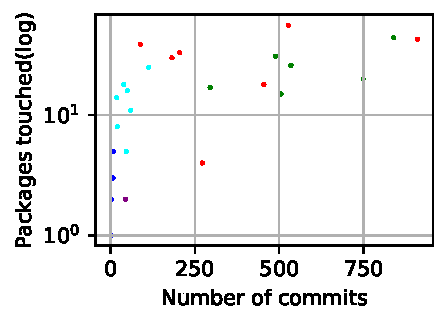
\includegraphics[width=\textwidth]{sections/results/21/packages/sample_scatter_touched_against_commit.packages.sample.first.pdf}
\vskip 5pt
{\small packages}
\label{figure.24.00000000000003}
\end{minipage}%
\hfill
  \vfill
\begin{minipage}[b]({0.45\textwidth})
\centering
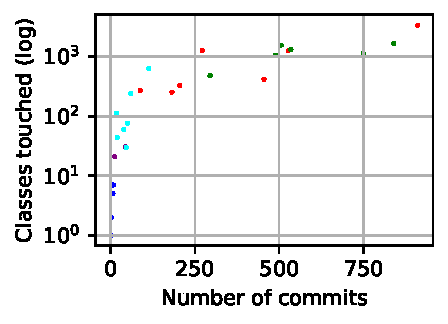
\includegraphics[width=\textwidth]{sections/results/21/classes/sample_scatter_touched_against_commit.classes.sample.first.pdf}
\vskip 5pt
{\small classes}
\label{figure.30.10000000000006}
\end{minipage}%
\hfill
\begin{minipage}[b]({0.45\textwidth})
\centering
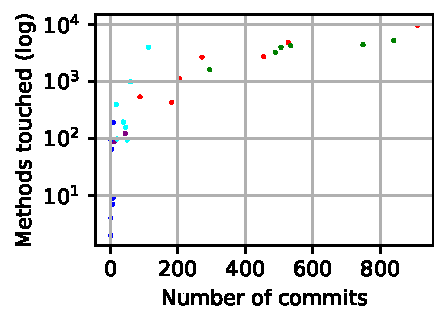
\includegraphics[width=\textwidth]{sections/results/21/methods/sample_scatter_touched_against_commit.methods.sample.first.pdf}
\vskip 5pt
{\small methods}
\label{figure.34.20000000000009}
\end{minipage}%
\hfill
\caption[Short]{\begin{minipage}[t]{\linewidth}Scatter plots of the log total number of components touched (y-axis) against the number of commits (x-axis) made by samples of developers capped at 84 sustained later joiners from six (6) categories: \color{Blue}Transient Founder (Blue, NUM1), \color{Purple}Moderate Founder (Purple, 3), \color{Green} Sustained Founder (Green, 7), \color{Orange} Transient Later Joiner (Orange, 84), \color{Cyan}Moderate Later Joiner (Cyan, 84), \color{Red} Sustained Later Joiner (Red, 84). \color{Black}\end{minipage}} 
\end{figure}
\newpage 
\subsection{Sample scatter touched against commit - Repository: 21} 
\begin{figure}[!htbp]
  \centering 
\begin{minipage}[b]{0.45\textwidth}
    \centering
    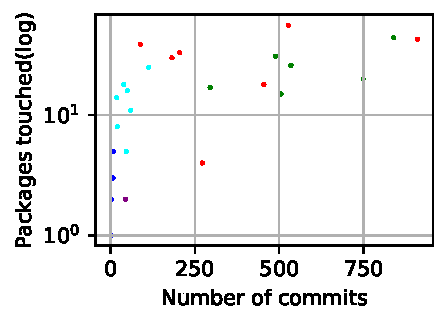
\includegraphics[width=\textwidth]{ sections/results/21/packages/sample_scatter_touched_against_commit.packages.sample.first.pdf }
    \vskip 5pt
    {\small packages}
    \label{ figure.24.00000000000003 }
\end{minipage}%
\hfill
  \vfill
\begin{minipage}[b]{0.45\textwidth}
    \centering
    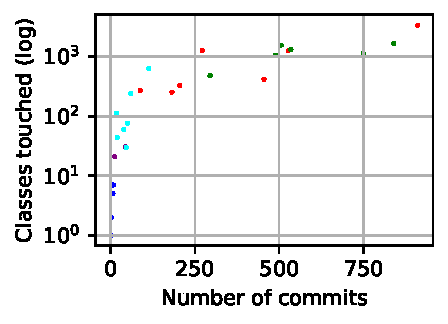
\includegraphics[width=\textwidth]{ sections/results/21/classes/sample_scatter_touched_against_commit.classes.sample.first.pdf }
    \vskip 5pt
    {\small classes}
    \label{ figure.30.10000000000006 }
\end{minipage}%
\hfill
\begin{minipage}[b]{0.45\textwidth}
    \centering
    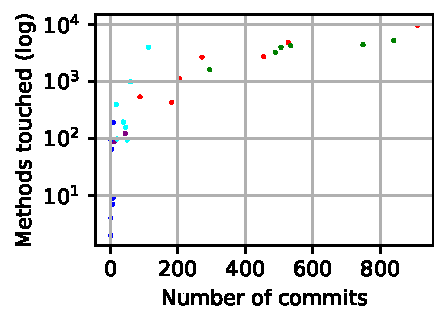
\includegraphics[width=\textwidth]{ sections/results/21/methods/sample_scatter_touched_against_commit.methods.sample.first.pdf }
    \vskip 5pt
    {\small methods}
    \label{ figure.34.20000000000009 }
\end{minipage}%
\hfill
\caption[Short]{\begin{minipage}[t]{\linewidth}Scatter plots of the log total number of components touched (y-axis) against the number of commits (x-axis) made by samples of developers capped at 84 sustained later joiners from six (6) categories: \color{Blue}Transient Founder (Blue, NUM1), \color{Purple}Moderate Founder (Purple, 3), \color{Green} Sustained Founder (Green, 7), \color{Orange} Transient Later Joiner (Orange, 84), \color{Cyan}Moderate Later Joiner (Cyan, 84), \color{Red} Sustained Later Joiner (Red, 84). \color{Black}\end{minipage}} 
\end{figure}
\newpage 
\subsection{Sample scatter touched against commit - Repository: 21} 
\begin{figure}[!htbp]
  \centering 
\begin{minipage}[b]{0.45\textwidth}
    \centering
    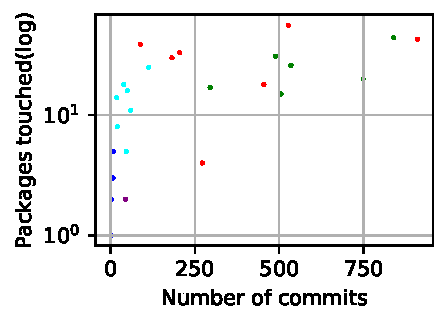
\includegraphics[width=\textwidth]{ sections/results/21/packages/sample_scatter_touched_against_commit.packages.sample.first.pdf }
    \vskip 5pt
    {\small packages}
    \label{ figure.24.00000000000003 }
\end{minipage}%
\hfill
  \vfill
\begin{minipage}[b]{0.45\textwidth}
    \centering
    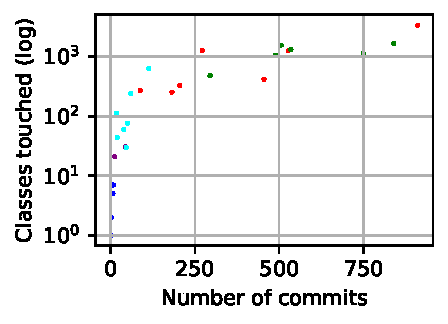
\includegraphics[width=\textwidth]{ sections/results/21/classes/sample_scatter_touched_against_commit.classes.sample.first.pdf }
    \vskip 5pt
    {\small classes}
    \label{ figure.30.10000000000006 }
\end{minipage}%
\hfill
\begin{minipage}[b]{0.45\textwidth}
    \centering
    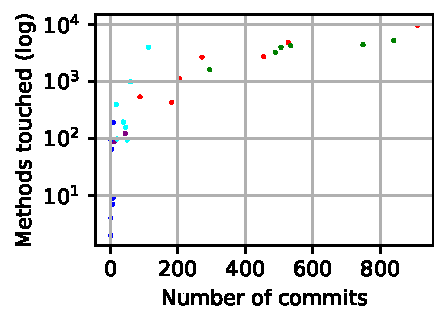
\includegraphics[width=\textwidth]{ sections/results/21/methods/sample_scatter_touched_against_commit.methods.sample.first.pdf }
    \vskip 5pt
    {\small methods}
    \label{ figure.34.20000000000009 }
\end{minipage}%
\hfill
\caption[Short]{\begin{minipage}[t]{\linewidth}Scatter plots of the log total number of components touched (y-axis) against the number of commits (x-axis) made by samples of developers capped at 84 sustained later joiners from six (6) categories: \color{Blue}Transient Founder (Blue, NUM1), \color{Purple}Moderate Founder (Purple, 3), \color{Green} Sustained Founder (Green, 7), \color{Orange} Transient Later Joiner (Orange, 84), \color{Cyan}Moderate Later Joiner (Cyan, 84), \color{Red} Sustained Later Joiner (Red, 84). \color{Black}\end{minipage}} 
\end{figure}
\newpage 
